\documentclass[tikz, border=10pt]{standalone}
\usepackage{tikz}
\usepackage{amsmath}
\usetikzlibrary{decorations.pathreplacing}
\begin{document}
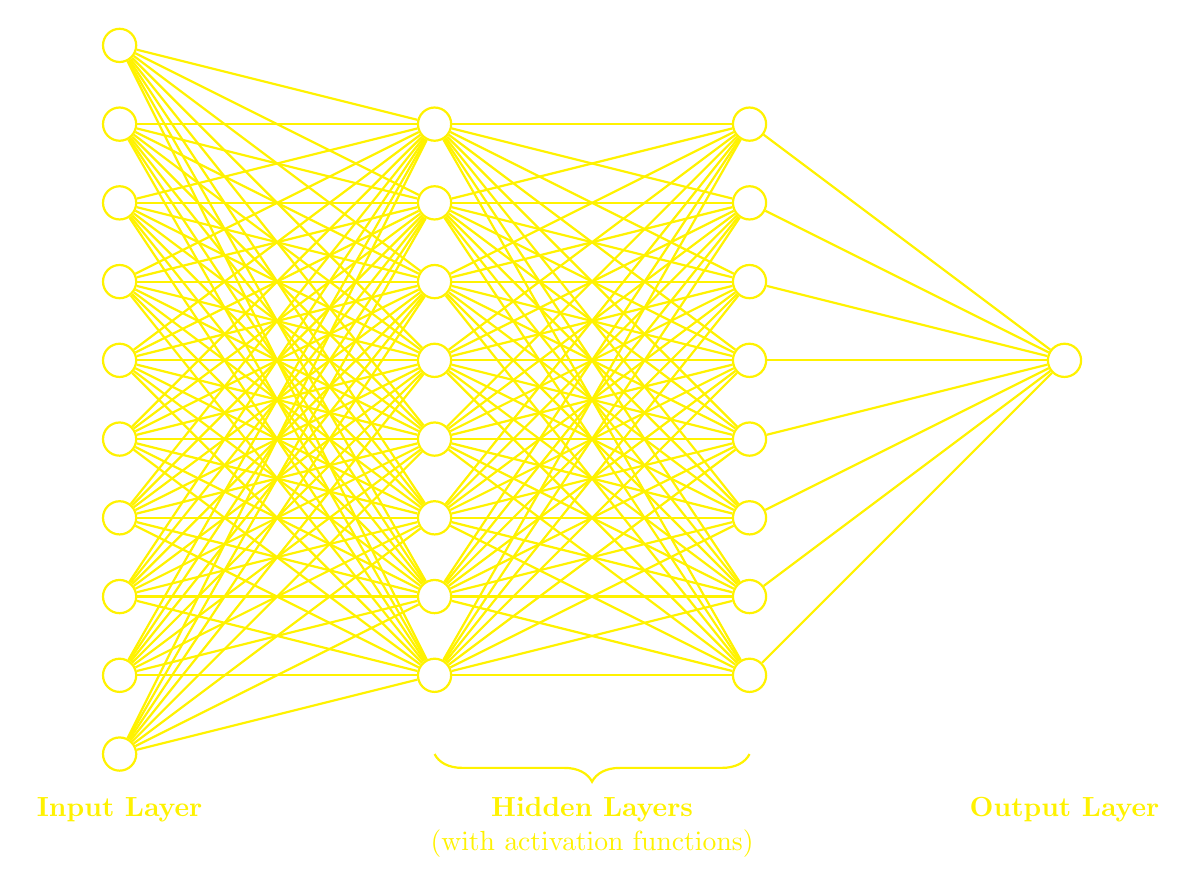
\begin{tikzpicture}[shorten >=0pt, draw=yellow, thick, every node/.style={text=yellow},]  % Removed spacing at the ends of lines
    \tikzstyle{neuron}=[circle, minimum size=12pt, draw=yellow, thick, fill=none]  % Circles with yellow boundary
    \tikzstyle{input neuron}=[neuron];
    \tikzstyle{hidden neuron}=[neuron];
    \tikzstyle{output neuron}=[neuron];
    \tikzstyle{annot} = [text width=4em, text centered]

    % Input layer
    \foreach \y in {1,2,...,10}
        \node[input neuron] (I-\y) at (0,-\y) {};

    % Label input Layer
        \node[below=12pt] at (0, -10)  (InputLayer) {
            \textbf{Input Layer}
        };

    % Hidden layer 1
    \foreach \y in {1,2,...,8}
        \node[hidden neuron] (H1-\y) at (4,-\y-1) {}; 

    % Hidden layer 2
    \foreach \y in {1,2,...,8}
        \node[hidden neuron] (H2-\y) at (8,-\y-1) {}; 

    % Label hidden layers
    \draw[decorate,decoration={brace,mirror,amplitude=10pt}] (4, -10) -- (8,-10)
        node[midway,below=12pt, align=center]{\textbf{Hidden Layers} \\ (with activation functions)};

    % Output layer
    \node[output neuron] (O) at (12,-5) {};  

    % Label input Layer
    \node[below=12pt] at (12, -10)  (OutputLayer) {
            \textbf{Output Layer} 
        };


    % Connect input layer to hidden layer 1
    \foreach \source in {1,2,...,10}
        \foreach \dest in {1,2,...,8}
            \draw (I-\source) -- (H1-\dest);

    % Connect hidden layer 1 to hidden layer 2
    \foreach \source in {1,2,...,8}
        \foreach \dest in {1,2,...,8}
            \draw (H1-\source) -- (H2-\dest);

    % Connect hidden layer 2 to output layer
    \foreach \source in {1,2,...,8}
        \draw (H2-\source) -- (O);
\end{tikzpicture}
\end{document}



